%The paper size, font size and document type are defined in the following
\documentclass[a4paper,12pt]{article}

\usepackage[utf8]{inputenc}
\usepackage[T1]{fontenc}
\usepackage{lmodern}
\usepackage[english]{babel}

%useful special symbols:
\usepackage{amssymb}
\usepackage{latexsym}
\usepackage{amsmath}
\usepackage{amsthm}

%a useful package if you write url addresses:
\usepackage{url}

%packages for figures, tables and the code listing:
\usepackage{xcolor}
\usepackage{graphicx}
\usepackage{subcaption}
\usepackage{booktabs}
\usepackage{listings}
\usepackage{tikz}
\usepackage[hidelinks]{hyperref}

%smaller page margins (the values suggested in the course template)
\textheight=24.3cm
\topmargin=-1.8cm
\textwidth=16.7cm
\oddsidemargin=-0.3cm
\evensidemargin=0.0cm

\graphicspath{{../figures/}}

%numbers computed by ../code/clustering_tendency.py; a missing value prints as ??
% generated by code/clustering_tendency.py -- do not edit
\expandafter\def\csname val@N\endcsname{1000}
\expandafter\def\csname val@NBoundary\endcsname{7}
\expandafter\def\csname val@Emax\endcsname{5.151}
\expandafter\def\csname val@EmaxBig\endcsname{7.591}
\expandafter\def\csname val@UnifMean\endcsname{5.119}
\expandafter\def\csname val@UnifSd\endcsname{0.006}
\expandafter\def\csname val@UnifMin\endcsname{5.093}
\expandafter\def\csname val@UnifMeanBig\endcsname{7.168}
\expandafter\def\csname val@UnifSdBig\endcsname{0.018}
\expandafter\def\csname val@HistMinOne\endcsname{6}
\expandafter\def\csname val@HistMaxOne\endcsname{25}
\expandafter\def\csname val@LowTwo\endcsname{762}
\expandafter\def\csname val@HighTwo\endcsname{238}
\expandafter\def\csname val@GapTwo\endcsname{18}
\expandafter\def\csname val@NSim\endcsname{10\,000}
\expandafter\def\csname val@NPerm\endcsname{2\,000}
\expandafter\def\csname val@Back\endcsname{$\{0,2\}$}
\expandafter\def\csname val@Fwd\endcsname{$\{0,2\}$}
\expandafter\def\csname val@E012\endcsname{4.794}
\expandafter\def\csname val@H012\endcsname{3.8064}
\expandafter\def\csname val@Z012\endcsname{-56.5}
\expandafter\def\csname val@EBig012\endcsname{6.610}
\expandafter\def\csname val@ZBig012\endcsname{-30.8}
\expandafter\def\csname val@Empty012\endcsname{9}
\expandafter\def\csname val@Rel012\endcsname{93.1}
\expandafter\def\csname val@Diff012\endcsname{0.988}
\expandafter\def\csname val@D012-012\endcsname{+0.000}
\expandafter\def\csname val@D012-01\endcsname{-0.204}
\expandafter\def\csname val@D012-02\endcsname{+0.312}
\expandafter\def\csname val@D012-12\endcsname{+0.002}
\expandafter\def\csname val@D012-0\endcsname{-0.160}
\expandafter\def\csname val@D012-1\endcsname{-0.324}
\expandafter\def\csname val@D012-2\endcsname{+0.033}
\expandafter\def\csname val@E01\endcsname{4.998}
\expandafter\def\csname val@H01\endcsname{4.0084}
\expandafter\def\csname val@Z01\endcsname{-20.9}
\expandafter\def\csname val@EBig01\endcsname{7.045}
\expandafter\def\csname val@ZBig01\endcsname{-6.8}
\expandafter\def\csname val@Empty01\endcsname{0}
\expandafter\def\csname val@Rel01\endcsname{97.0}
\expandafter\def\csname val@Diff01\endcsname{0.990}
\expandafter\def\csname val@D01-012\endcsname{+0.204}
\expandafter\def\csname val@D01-01\endcsname{+0.000}
\expandafter\def\csname val@D01-02\endcsname{+0.516}
\expandafter\def\csname val@D01-12\endcsname{+0.206}
\expandafter\def\csname val@D01-0\endcsname{+0.044}
\expandafter\def\csname val@D01-1\endcsname{-0.120}
\expandafter\def\csname val@D01-2\endcsname{+0.237}
\expandafter\def\csname val@E02\endcsname{4.482}
\expandafter\def\csname val@H02\endcsname{3.5031}
\expandafter\def\csname val@Z02\endcsname{-110.7}
\expandafter\def\csname val@EBig02\endcsname{6.568}
\expandafter\def\csname val@ZBig02\endcsname{-33.1}
\expandafter\def\csname val@Empty02\endcsname{10}
\expandafter\def\csname val@Rel02\endcsname{87.0}
\expandafter\def\csname val@Diff02\endcsname{0.979}
\expandafter\def\csname val@D02-012\endcsname{-0.312}
\expandafter\def\csname val@D02-01\endcsname{-0.516}
\expandafter\def\csname val@D02-02\endcsname{+0.000}
\expandafter\def\csname val@D02-12\endcsname{-0.310}
\expandafter\def\csname val@D02-0\endcsname{-0.472}
\expandafter\def\csname val@D02-1\endcsname{-0.636}
\expandafter\def\csname val@D02-2\endcsname{-0.279}
\expandafter\def\csname val@E12\endcsname{4.792}
\expandafter\def\csname val@H12\endcsname{3.8060}
\expandafter\def\csname val@Z12\endcsname{-56.8}
\expandafter\def\csname val@EBig12\endcsname{6.879}
\expandafter\def\csname val@ZBig12\endcsname{-15.9}
\expandafter\def\csname val@Empty12\endcsname{0}
\expandafter\def\csname val@Rel12\endcsname{93.0}
\expandafter\def\csname val@Diff12\endcsname{0.986}
\expandafter\def\csname val@D12-012\endcsname{-0.002}
\expandafter\def\csname val@D12-01\endcsname{-0.206}
\expandafter\def\csname val@D12-02\endcsname{+0.310}
\expandafter\def\csname val@D12-12\endcsname{+0.000}
\expandafter\def\csname val@D12-0\endcsname{-0.162}
\expandafter\def\csname val@D12-1\endcsname{-0.326}
\expandafter\def\csname val@D12-2\endcsname{+0.031}
\expandafter\def\csname val@E0\endcsname{4.954}
\expandafter\def\csname val@H0\endcsname{3.9651}
\expandafter\def\csname val@Z0\endcsname{-28.6}
\expandafter\def\csname val@EBig0\endcsname{7.020}
\expandafter\def\csname val@ZBig0\endcsname{-8.2}
\expandafter\def\csname val@Empty0\endcsname{0}
\expandafter\def\csname val@Rel0\endcsname{96.2}
\expandafter\def\csname val@Diff0\endcsname{0.989}
\expandafter\def\csname val@D0-012\endcsname{+0.160}
\expandafter\def\csname val@D0-01\endcsname{-0.044}
\expandafter\def\csname val@D0-02\endcsname{+0.472}
\expandafter\def\csname val@D0-12\endcsname{+0.162}
\expandafter\def\csname val@D0-0\endcsname{+0.000}
\expandafter\def\csname val@D0-1\endcsname{-0.164}
\expandafter\def\csname val@D0-2\endcsname{+0.193}
\expandafter\def\csname val@E1\endcsname{5.118}
\expandafter\def\csname val@H1\endcsname{4.1264}
\expandafter\def\csname val@Z1\endcsname{-0.1}
\expandafter\def\csname val@EBig1\endcsname{7.155}
\expandafter\def\csname val@ZBig1\endcsname{-0.7}
\expandafter\def\csname val@Empty1\endcsname{0}
\expandafter\def\csname val@Rel1\endcsname{99.4}
\expandafter\def\csname val@Diff1\endcsname{0.992}
\expandafter\def\csname val@D1-012\endcsname{+0.324}
\expandafter\def\csname val@D1-01\endcsname{+0.120}
\expandafter\def\csname val@D1-02\endcsname{+0.636}
\expandafter\def\csname val@D1-12\endcsname{+0.326}
\expandafter\def\csname val@D1-0\endcsname{+0.164}
\expandafter\def\csname val@D1-1\endcsname{+0.000}
\expandafter\def\csname val@D1-2\endcsname{+0.357}
\expandafter\def\csname val@E2\endcsname{4.761}
\expandafter\def\csname val@H2\endcsname{3.7757}
\expandafter\def\csname val@Z2\endcsname{-62.2}
\expandafter\def\csname val@EBig2\endcsname{6.867}
\expandafter\def\csname val@ZBig2\endcsname{-16.6}
\expandafter\def\csname val@Empty2\endcsname{1}
\expandafter\def\csname val@Rel2\endcsname{92.4}
\expandafter\def\csname val@Diff2\endcsname{0.986}
\expandafter\def\csname val@D2-012\endcsname{-0.033}
\expandafter\def\csname val@D2-01\endcsname{-0.237}
\expandafter\def\csname val@D2-02\endcsname{+0.279}
\expandafter\def\csname val@D2-12\endcsname{-0.031}
\expandafter\def\csname val@D2-0\endcsname{-0.193}
\expandafter\def\csname val@D2-1\endcsname{-0.357}
\expandafter\def\csname val@D2-2\endcsname{+0.000}
\expandafter\def\csname val@R01\endcsname{0.035}
\expandafter\def\csname val@MI01\endcsname{0.021}
\expandafter\def\csname val@MINull01\endcsname{0.025}
\expandafter\def\csname val@R02\endcsname{0.152}
\expandafter\def\csname val@MI02\endcsname{0.208}
\expandafter\def\csname val@MINull02\endcsname{0.026}
\expandafter\def\csname val@R12\endcsname{0.054}
\expandafter\def\csname val@MI12\endcsname{0.029}
\expandafter\def\csname val@MINull12\endcsname{0.025}
\expandafter\def\csname val@SizeA\endcsname{511}
\expandafter\def\csname val@CentreA\endcsname{(0.25, 0.25)}
\expandafter\def\csname val@SizeB\endcsname{251}
\expandafter\def\csname val@CentreB\endcsname{(0.74, 0.25)}
\expandafter\def\csname val@SizeC\endcsname{238}
\expandafter\def\csname val@CentreC\endcsname{(0.51, 0.75)}
\expandafter\def\csname val@BackSh\endcsname{$\{0,2\}$}
\expandafter\def\csname val@FwdSh\endcsname{$\{0,2\}$}
\expandafter\def\csname val@BackBig\endcsname{$\{0,2\}$}
\expandafter\def\csname val@FwdBig\endcsname{$\{0,2\}$}

\newcommand{\val}[1]{\ifcsname val@#1\endcsname\csname val@#1\endcsname\else\textbf{??}\fi}
\newcommand{\ent}[1]{\val{E#1}}                %entropy of a set of dimensions, e.g. \ent{02}
\newcommand{\dE}[2]{\val{D#1-#2}}              %difference E(#1) - E(#2)
\newcommand{\dims}[1]{\ensuremath{\{#1\}}}     %a set of dimensions, e.g. \dims{0,2}

\lstset{language=Python, basicstyle=\ttfamily\scriptsize, numbers=left,
  numberstyle=\tiny\color{gray}, breaklines=true, columns=fullflexible,
  keepspaces=true, showstringspaces=false, upquote=true, frame=tb,
  rulecolor=\color{gray},
  keywordstyle=\color{blue!60!black}, commentstyle=\color{green!40!black},
  stringstyle=\color{red!50!black}}

%>>> fill in the homework number and the team before submitting <<<
\newcommand{\hwnumber}{N}
\title{CS-E4650 Methods of Data Mining, Homework \hwnumber\\[1ex]
  \large Clustering tendency and entropy-based measures}
\author{Student Name (student id 000000) and Student Name (student id 000000)}

\begin{document}

\maketitle

%---------------------------------------------------------------------------
\section{Methods}

All computations were made in Python~3.11 with NumPy~2.4 (loading and
checking the data, discretisation, entropies, greedy searches and
simulations) and Matplotlib~3.11 (figures); the report was written in
\LaTeX{} with the course template. The script in the Appendix reproduces
every figure, table and number of this report. We first verified that
the data file contains \val{N} three-dimensional vectors whose values all
lie in $[0,1]$ (the smallest value is exactly 0 and the largest exactly 1;
\val{NBoundary} values lie on the boundary). For every non-empty subset
of $k$ dimensions, the cube $[0,1]^k$ was divided into $m=64$ equal cells
by splitting each of its dimensions into $64^{1/k}$ equal ranges, the
fraction of points in each cell was counted, and the probability-based
entropy of equation~(6.2) of Aggarwal's book~\cite{aggarwal} was computed
(Section~\ref{sec:entropies}). The greedy backward and forward searches
were simulated on the seven resulting entropy values. Beyond the required
experiments we made four small extra experiments, reported in
Section~\ref{sec:extra}: (i)~the plain Shannon entropy instead of
equation~(6.2), (ii)~a Monte Carlo baseline of the entropy of uniformly
distributed data (\val{NSim} simulated data sets), (iii)~the correlation
and mutual information of each pair of components with a permutation test
of independence, and (iv)~all entropies and both greedy searches with
$m=729$ cells.

%---------------------------------------------------------------------------
\section{Histograms}\label{sec:histograms}

Figure~\ref{fig:hist} shows the histograms of the three components with 64
equal-width bins on $[0,1]$; these bins are the same 64 ranges that are
used for the one-dimensional entropies. The dashed line marks the count
$1000/64\approx15.6$ that is expected in every bin if a component is
uniformly distributed.

\begin{figure}[!ht]
\centering
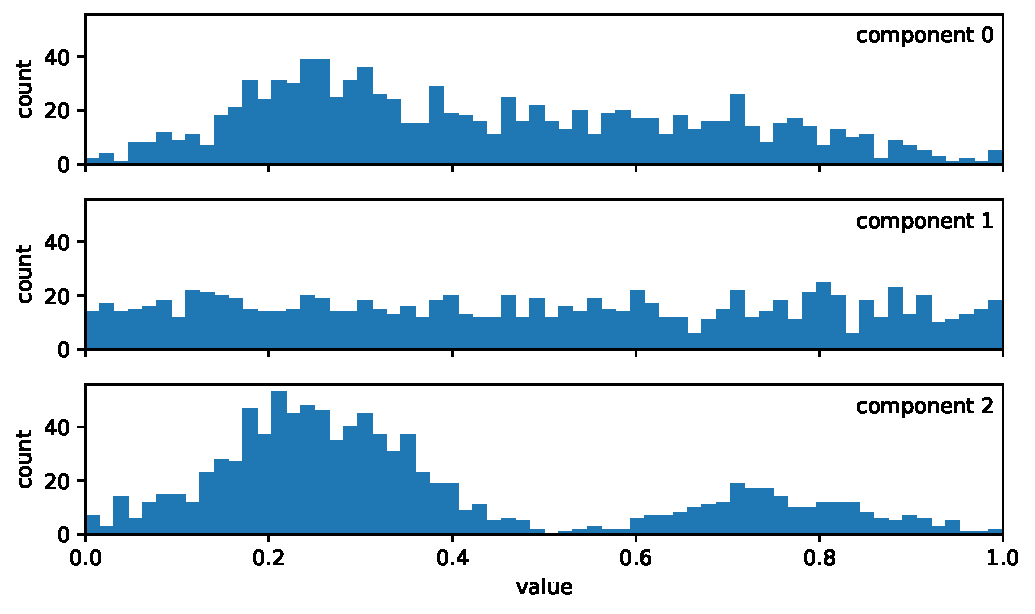
\includegraphics[width=0.95\textwidth]{histograms.pdf}
\caption{Histograms (64 bins) of component~0 (top), component~1 (middle)
  and component~2 (bottom). All panels share the same count axis. Dashed
  line: expected count per bin for a uniform distribution.}
\label{fig:hist}
\end{figure}

\begin{description}
\item[Component 0] is unimodal but strongly skewed: a pronounced peak at
  about 0.2--0.3 is followed by a broad shoulder that extends to about
  0.9, and both tails are thin. The distribution is clearly not uniform,
  and the combination of a narrow peak with a wide plateau hints at
  several overlapping groups, but there is no empty region that would
  separate them. On its own, component~0 therefore shows only a weak
  clustering tendency: the points cannot be split into well-separated
  groups along this axis.
\item[Component 1] is flat. The bin counts fluctuate between
  \val{HistMinOne} and \val{HistMaxOne} around the uniform level without
  systematic peaks or gaps, which is what random sampling from a uniform
  distribution produces. Component~1 shows no clustering tendency at all.
\item[Component 2] is clearly bimodal. A large mode around 0.25 holds
  about three quarters of the points (\val{LowTwo} values below 0.5), a
  smaller mode around 0.75 holds the rest (\val{HighTwo}), and between
  them there is an almost empty gap (only \val{GapTwo} values in
  $[0.45,0.55)$). Component~2 alone already shows a strong clustering
  tendency with two natural groups.
\end{description}

\noindent Judged by these one-dimensional views alone, component~2 would
contribute most to the clustering tendency, component~0 somewhat, and
component~1 not at all.

%---------------------------------------------------------------------------
\section{Scatter plots}\label{sec:scatter}

Figure~\ref{fig:scatter} shows the scatter plots of the three pairs of
components with equal scales on both axes. The light grey lines mark the
$8\times8$ grid that is used for the two-dimensional entropies.

\begin{figure}[!ht]
\centering
\begin{subfigure}[b]{0.32\textwidth}\centering
  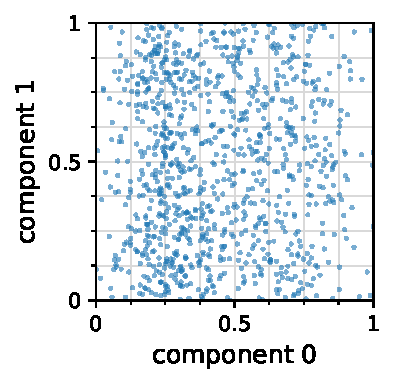
\includegraphics[width=\textwidth]{scatter_0_1.pdf}
  \caption{components 0 and 1}\label{fig:sc01}
\end{subfigure}\hfill
\begin{subfigure}[b]{0.32\textwidth}\centering
  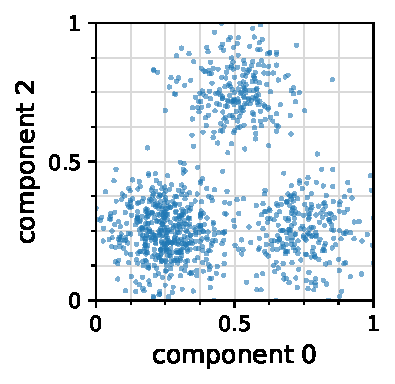
\includegraphics[width=\textwidth]{scatter_0_2.pdf}
  \caption{components 0 and 2}\label{fig:sc02}
\end{subfigure}\hfill
\begin{subfigure}[b]{0.32\textwidth}\centering
  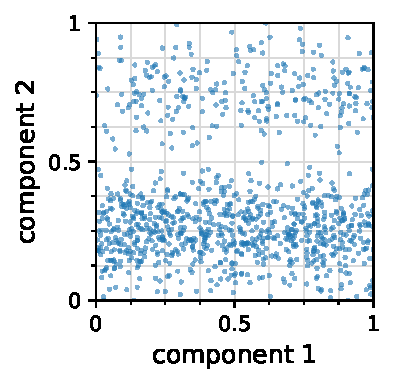
\includegraphics[width=\textwidth]{scatter_1_2.pdf}
  \caption{components 1 and 2}\label{fig:sc12}
\end{subfigure}
\caption{Scatter plots of the three pairs of components with equal aspect
  ratio; each axis is labelled with the component it shows. Grey lines:
  the $8\times8$ grid of the two-dimensional entropy calculation.}
\label{fig:scatter}
\end{figure}

\paragraph{Components 0 and 1 (Figure~\ref{fig:sc01}).} The points fill
the whole square without any groups. The density changes only along
component~0 (a denser vertical band at 0.15--0.35 that thins out towards
1), and this pattern is the same at every value of component~1. The joint
distribution thus looks like the product of the two marginal
distributions: the components appear independent (Pearson correlation
$r=\val{R01}$, and the mutual information is at the level of independent
data, Section~\ref{sec:extra}). Combining the uniform component~1 with
component~0 only spreads the points out; it does not create clusters.

\paragraph{Components 0 and 2 (Figure~\ref{fig:sc02}).} Three compact,
well-separated clusters appear: a large one around \val{CentreA} with
about half of the points (\val{SizeA}), and two smaller ones around
\val{CentreB} (\val{SizeB} points) and \val{CentreC} (\val{SizeC}
points).\footnote{Coordinates are given as (component~0, component~2);
the sizes and centres were obtained by splitting the plane at 0.5 in both
components.} The two components are strongly dependent: when component~2
is low, component~0 is bimodal (around 0.25 or 0.75), and when
component~2 is high, component~0 is concentrated around 0.5. The
dependence is not linear ($r=\val{R02}$ only), but the mutual information
is about eight times the level of independent data
(Section~\ref{sec:extra}). As a consequence, neither one-dimensional
projection shows all three clusters: in component~2 the two lower
clusters coincide, and in component~0 the upper cluster falls between the
two lower ones and fills the gap between them, which explains why the
histogram of component~0 has no gap. Only the combination of components~0
and~2 reveals the full cluster structure, so the pair has a clearly
stronger clustering tendency than either of its components alone.

\paragraph{Components 1 and 2 (Figure~\ref{fig:sc12}).} The points form
two horizontal bands, at component~2 $\approx0.25$ and $\approx0.75$, that
extend evenly over the whole range of component~1. This is simply the
bimodality of component~2 seen together with a uniform, independent
component~1 ($r=\val{R12}$, mutual information at the independence
level). The two lower clusters merge into one band, so only two groups are
visible.

\medskip\noindent In summary, component~1 is uniformly distributed and
independent of the other two components: it is a noise dimension that
carries no cluster information. If it is included, every cluster is
stretched into a ``rod'' along the whole component-1 axis, so points of
the same cluster can be far apart in the full space and the clusters
become much less compact. Components~0 and~2, in contrast, depend on each
other, and the clusters live in their joint subspace.

%---------------------------------------------------------------------------
\section{Entropies}\label{sec:entropies}

For a subset of $k$ dimensions, each dimension was divided into
$\varphi=64^{1/k}$ equal ranges ($\varphi=4$, 8 and 64 for $k=3$, 2 and
1), so that every grid has exactly $m=64$ cells. A value $x$ was assigned
to range $\lfloor\varphi x\rfloor$ and the value $x=1$ to the last range,
so that the grid covers the closed cube $[0,1]^k$. With $p_i$ the fraction
of the 1000 points in cell~$i$, the probability-based entropy of
equation~(6.2) in~\cite{aggarwal} is
\begin{equation}
  E=-\sum_{i=1}^{m}\bigl[p_i\ln p_i+(1-p_i)\ln(1-p_i)\bigr],
  \label{eq:entropy}
\end{equation}
computed with the natural logarithm and $0\ln0=0$. Because $m$ is the same
for all subsets, all values share the same scale: $E=0$ if all points fall
into one cell, and the maximum
$E_{\max}=\ln64-63\ln\frac{63}{64}\approx\val{Emax}$ is reached when every
cell holds the same fraction $p_i=1/64$. A sample of 1000 uniformly
distributed points gives $E=\val{UnifMean}\pm\val{UnifSd}$ (mean $\pm$
standard deviation, Section~\ref{sec:extra}), slightly below $E_{\max}$
because of random fluctuations. Table~\ref{tab:entropies} lists the seven
entropies.

\begin{table}[!ht]
\centering
\caption{Probability-based entropies $E$ (equation~(\ref{eq:entropy}),
  $m=64$ cells) of all combinations of data dimensions. Grid: ranges per
  dimension; empty cells: cells without any point; $E/E_{\max}$: entropy
  relative to its maximum $E_{\max}=\val{Emax}$; rank~1 is the lowest
  entropy.}
\label{tab:entropies}
\begin{tabular}{lcccccc}
\toprule
Dimensions & $k$ & Grid & Empty cells & $E$ & $E/E_{\max}$ & Rank \\
\midrule
$\{0,1,2\}$ & 3 & $4\times4\times4$ & 9 & 4.794 & 93.1\,\% & 4 \\
\midrule
$\{0,1\}$ & 2 & $8\times8$ & 0 & 4.998 & 97.0\,\% & 6 \\
$\{0,2\}$ & 2 & $8\times8$ & 10 & 4.482 & 87.0\,\% & 1 \\
$\{1,2\}$ & 2 & $8\times8$ & 0 & 4.792 & 93.0\,\% & 3 \\
\midrule
$\{0\}$ & 1 & $64$ & 0 & 4.954 & 96.2\,\% & 5 \\
$\{1\}$ & 1 & $64$ & 0 & 5.118 & 99.4\,\% & 7 \\
$\{2\}$ & 1 & $64$ & 1 & 4.761 & 92.4\,\% & 2 \\
\bottomrule
\end{tabular}

\end{table}

\paragraph{Range and variation.} The seven values lie in the narrow
interval \ent{02}--\ent{1}, i.e.\ \val{Rel02}--\val{Rel1}\,\% of
$E_{\max}$. In absolute terms the differences look small, but they are
large compared with the random variation of the entropy of uniform data
(standard deviation \val{UnifSd}): apart from \dims{1,2} and \dims{0,1,2},
which differ by only $\dE{012}{12}$, any two values differ by more than
five such standard deviations. Since a low entropy means that the points
are concentrated in few cells instead of being spread evenly, the ranking
\[
  E_{\{0,2\}}<E_{\{2\}}<E_{\{1,2\}}\approx E_{\{0,1,2\}}<E_{\{0\}}
  <E_{\{0,1\}}<E_{\{1\}}
\]
orders the combinations from the strongest to the weakest clustering
tendency.

\paragraph{What the values indicate about the components.}
\begin{itemize}
\item \dims{0,2} has by far the lowest entropy (\ent{02}), and
  \val{Empty02} of its 64 cells are empty: the regions between the three
  clusters. This is the combination with the strongest clustering
  tendency.
\item Component~1 has the highest entropy, $E_{\{1\}}=\ent{1}$,
  practically equal to that of uniform random data
  ($\val{UnifMean}\pm\val{UnifSd}$). Moreover, adding component~1 to any
  subset increases the entropy: $E_{\{0,1\}}-E_{\{0\}}=\dE{01}{0}$,
  $E_{\{1,2\}}-E_{\{2\}}=\dE{12}{2}$ and
  $E_{\{0,1,2\}}-E_{\{0,2\}}=\dE{012}{02}$. Because $m$ is fixed, a new
  dimension brings no new cells but divides the existing resolution: a
  uniform, independent component spreads the points of every coarser cell
  evenly over several finer cells and therefore raises the entropy.
  Component~1 contributes nothing to the clustering tendency; it even
  masks the structure of the other components.
\item Component~2 has the lowest single-dimension entropy (\ent{2}), and
  adding it always decreases the entropy:
  $E_{\{0,2\}}-E_{\{0\}}=\dE{02}{0}$, $E_{\{1,2\}}-E_{\{1\}}=\dE{12}{1}$
  and $E_{\{0,1,2\}}-E_{\{0,1\}}=\dE{012}{01}$. It is the strongest
  individual contributor.
\item Component~0 has an intermediate single entropy (\ent{0}): clearly
  below the uniform level but well above component~2, so on its own it
  contributes moderately. Together with component~2 it contributes a lot,
  $E_{\{0,2\}}-E_{\{2\}}=\dE{02}{2}$: the pair is more than the sum of its
  parts. In the three-dimensional grid, however, adding component~0 to
  \dims{1,2} changes the entropy by only $\dE{012}{12}$, a resolution
  effect discussed in Section~\ref{sec:analysis}.
\end{itemize}

%---------------------------------------------------------------------------
\section{Greedy backward selection}\label{sec:backward}

Backward selection starts from the full set of dimensions and at each
stage removes the dimension whose removal gives the lowest entropy, as
long as this lowers the entropy; following Aggarwal~\cite{aggarwal}, the
search stops when the entropy would increase (or not decrease
significantly). Table~\ref{tab:backward} and
Figure~\ref{fig:lattice}(a) show the stages.

\begin{table}[!ht]
\centering
\caption{Stages of greedy backward selection. $\Delta E$: change of the
  entropy relative to the current set; bold: lowest entropy of the stage.}
\label{tab:backward}
\begin{tabular}{cllrrl}
\toprule
Stage & Current set ($E$) & Candidate set & $E$ & $\Delta E$ & Decision \\
\midrule
1 & $\{0,1,2\}$ (4.794) & $\{1,2\}$ (remove 0) & 4.792 & $-0.002$ &  \\
& & $\{0,2\}$ (remove 1) & \textbf{4.482} & $-0.312$ & selected \\
& & $\{0,1\}$ (remove 2) & 4.998 & $+0.204$ &  \\
\midrule
2 & $\{0,2\}$ (4.482) & $\{2\}$ (remove 0) & \textbf{4.761} & $+0.279$ & stop: $E$ would increase \\
& & $\{0\}$ (remove 2) & 4.954 & $+0.472$ &  \\
\bottomrule
\end{tabular}

\end{table}

\begin{description}
\item[Stage 1.] Starting from \dims{0,1,2} with $E=\ent{012}$, the three
  possible removals give \dims{1,2} (\ent{12}), \dims{0,2} (\ent{02}) and
  \dims{0,1} (\ent{01}). Removing component~1 gives by far the largest
  reduction ($\dE{02}{012}$), so component~1 is dropped. Removing
  component~0 would lower the entropy only marginally ($\dE{12}{012}$),
  and removing component~2 would increase it ($\dE{01}{012}$).
\item[Stage 2.] From \dims{0,2} ($E=\ent{02}$), removing component~0
  gives \dims{2} with \ent{2} and removing component~2 gives \dims{0}
  with \ent{0}. Both would increase the entropy (by $\dE{2}{02}$ and
  $\dE{0}{02}$), so the search stops.
\end{description}
The result is \val{Back} with $E=\ent{02}$. The search evaluated six of the
seven subsets; only \dims{1} was never computed.

\begin{figure}[!ht]
\centering
\tikzset{
  sub/.style={draw, rounded corners=2pt, align=center, font=\footnotesize,
    minimum width=15mm, inner sep=2pt, fill=white},
  noeval/.style={sub, dashed, draw=gray, text=gray},
  result/.style={sub, very thick, fill=green!12},
  link/.style={gray!50},
  move/.style={-latex, very thick, blue!70!black},
  halt/.style={-latex, thick, dashed, red!75!black},
}
\begin{subfigure}[b]{0.49\textwidth}\centering
\begin{tikzpicture}[x=21mm, y=15mm]
  \path[use as bounding box] (-0.5,-1.35) rectangle (2.5,2.35);
  \node[sub]    (a012) at (1,2) {\dims{0,1,2}\\\ent{012}};
  \node[sub]    (a01)  at (0,1) {\dims{0,1}\\\ent{01}};
  \node[result] (a02)  at (1,1) {\dims{0,2}\\\ent{02}};
  \node[sub]    (a12)  at (2,1) {\dims{1,2}\\\ent{12}};
  \node[sub]    (a0)   at (0,0) {\dims{0}\\\ent{0}};
  \node[noeval] (a1)   at (1,0) {\dims{1}\\\ent{1}};
  \node[sub]    (a2)   at (2,0) {\dims{2}\\\ent{2}};
  \foreach \u/\v in {a012/a01, a012/a12, a01/a0, a01/a1, a02/a0, a12/a1, a12/a2}
    \draw[link] (\u) -- (\v);
  \draw[move] (a012) -- (a02);
  \draw[halt] (a02) -- (a2);
\end{tikzpicture}
\caption{backward selection}
\end{subfigure}\hfill
\begin{subfigure}[b]{0.49\textwidth}\centering
\begin{tikzpicture}[x=21mm, y=15mm]
  \path[use as bounding box] (-0.5,-1.35) rectangle (2.5,2.35);
  \node[sub]    (b012) at (1,2) {\dims{0,1,2}\\\ent{012}};
  \node[noeval] (b01)  at (0,1) {\dims{0,1}\\\ent{01}};
  \node[result] (b02)  at (1,1) {\dims{0,2}\\\ent{02}};
  \node[sub]    (b12)  at (2,1) {\dims{1,2}\\\ent{12}};
  \node[sub]    (b0)   at (0,0) {\dims{0}\\\ent{0}};
  \node[sub]    (b1)   at (1,0) {\dims{1}\\\ent{1}};
  \node[sub]    (b2)   at (2,0) {\dims{2}\\\ent{2}};
  \node[sub]    (be)   at (1,-1) {$\emptyset$};
  \foreach \u/\v in {b012/b01, b012/b12, b01/b0, b01/b1, b02/b0, b12/b1, b12/b2,
      be/b0, be/b1}
    \draw[link] (\u) -- (\v);
  \draw[move] (be) -- (b2);
  \draw[move] (b2) -- (b02);
  \draw[halt] (b02) -- (b012);
\end{tikzpicture}
\caption{forward selection}
\end{subfigure}
\caption{All subsets of dimensions with their entropies $E$ and the paths
  of the two greedy searches. Solid blue arrows: accepted steps; dashed
  red arrow: best move of the last stage, rejected because $E$ would
  increase; dashed grey box: subset never evaluated by the search; green
  box: result. Grey lines connect subsets that differ by one dimension.}
\label{fig:lattice}
\end{figure}

%---------------------------------------------------------------------------
\section{Greedy forward selection}\label{sec:forward}

Forward selection starts from the empty set and at each stage adds the
dimension that gives the lowest entropy, as long as this lowers the
entropy. Table~\ref{tab:forward} and Figure~\ref{fig:lattice}(b) show the
stages.

\begin{table}[!ht]
\centering
\caption{Stages of greedy forward selection. $\Delta E$: change of the
  entropy relative to the current set; bold: lowest entropy of the stage.}
\label{tab:forward}
\begin{tabular}{cllrrl}
\toprule
Stage & Current set ($E$) & Candidate set & $E$ & $\Delta E$ & Decision \\
\midrule
1 & $\emptyset$ & $\{0\}$ (add 0) & 4.954 & -- &  \\
& & $\{1\}$ (add 1) & 5.118 & -- &  \\
& & $\{2\}$ (add 2) & \textbf{4.761} & -- & selected \\
\midrule
2 & $\{2\}$ (4.761) & $\{0,2\}$ (add 0) & \textbf{4.482} & $-0.279$ & selected \\
& & $\{1,2\}$ (add 1) & 4.792 & $+0.031$ &  \\
\midrule
3 & $\{0,2\}$ (4.482) & $\{0,1,2\}$ (add 1) & \textbf{4.794} & $+0.312$ & stop: $E$ would increase \\
\bottomrule
\end{tabular}

\end{table}

\begin{description}
\item[Stage 1.] The empty set has no entropy on a 64-cell grid (all points
  would lie in a single cell), so the first stage simply takes the best
  single dimension: component~2 (\ent{2}), ahead of component~0
  (\ent{0}) and component~1 (\ent{1}).
\item[Stage 2.] Adding component~0 gives \dims{0,2} with \ent{02}
  ($\dE{02}{2}$), adding component~1 gives \dims{1,2} with \ent{12}
  ($\dE{12}{2}$). Component~0 is added.
\item[Stage 3.] The only remaining option, adding component~1, would
  increase the entropy to \ent{012} ($\dE{012}{02}$), so the search stops.
\end{description}
The result is \val{Fwd} with $E=\ent{02}$, the same as in backward
selection. Again six of the seven subsets were evaluated; this time
\dims{0,1} was never computed.

%---------------------------------------------------------------------------
\section{Analysis}\label{sec:analysis}

\paragraph{A consistent picture.} The visual inspection suggested that the
clusters live in the plane of components~0 and~2 and that component~1 is
uniform noise. The entropies confirm this: \dims{0,2} has the lowest
entropy, \dims{1} is at the level of uniform data, and every subset with
component~1 has a higher entropy than the same subset without it. Both
greedy searches end at \dims{0,2}, which is also the minimum of all seven
values, i.e.\ the result an exhaustive search would give. This is what we
expected from the plots. The decisive steps are also robust: the entropy
changes of the accepted moves (0.28--0.31) are about fifty times the
standard deviation of the entropy of uniform data, and the result stays
the same with the Shannon entropy and with $m=729$
(Section~\ref{sec:extra}).

\paragraph{Why the two strategies agree here.} The structure of these data
is easy for greedy search. Component~1 is harmful in every combination, so
backward selection removes it first, and components~0 and~2 are
informative both individually and together, so forward selection builds
\dims{0,2} step by step. The two directions therefore meet at the same
subset. In general this is not guaranteed: a greedy search never revisits
a decision, and forward and backward selection can end at different
subsets, neither of which needs to be optimal.

\paragraph{Where the greedy searches could fail.} Forward selection judges
each component first on its own. Our data contain a mild example of why
this is risky: component~0 alone looks only weakly clustered (no gap in
the histogram, $E_{\{0\}}=\ent{0}$), yet it is essential for separating
the two lower clusters, which is visible only together with component~2.
Forward selection found it because component~0 is not completely uniform
and because in stage~2 it was evaluated together with component~2. If two
components were uniform individually but clustered jointly (for example
in a checkerboard pattern), forward selection would start from some other
component and could miss the pair, whereas backward selection, which
starts from the full space, can still detect the joint structure. Backward
selection, on the other hand, makes its first decision on the coarsest
grid, where the entropies are least informative, as the next paragraph
shows.

\paragraph{The entropy depends on the resolution.} Although the three
clusters exist in the full space, the entropy of \dims{0,1,2} (\ent{012})
is higher than those of \dims{0,2} and \dims{2} and practically equal to
that of \dims{1,2}; adding component~0 to \dims{1,2} does not lower the
entropy at all ($\dE{012}{12}$). With $m$ fixed, every added dimension
lowers the resolution of all dimensions (64, 8 and 4 ranges for $k=1$, 2
and 3). In the $4\times4\times4$ grid the range boundaries 0.25, 0.5 and
0.75 run right through the cluster centres (Section~\ref{sec:scatter}), so
each cluster is split over $2\times2$ cells of the (0,\,2)-plane, and the
uniform component~1 divides each of these cells further into four almost
equally filled cells. The entropies therefore compare not only the data
but also the grid resolutions, and comparisons across dimensionalities,
which the stopping rules of both searches make, must be read with care. In
our data this did not matter because removing component~1 was clearly the
best first step, but with a less harmful noise component the coarse grid
could have made backward selection drop component~0, a decision it could
never undo.

\paragraph{Low entropy is not the same as clusters.} The entropy measures
how unevenly the points are spread over the cells, not whether they form
separate groups. Component~0 has an entropy far below the uniform level
($z=\val{Z0}$ in Section~\ref{sec:extra}) mainly because its distribution
is skewed, although its histogram shows no separated groups; a single
dense blob would likewise have a low entropy. Visual inspection is needed
to tell whether a low entropy comes from several separated groups or
merely from a non-uniform density. In our data the low entropy of
\dims{0,2} does correspond to three real clusters, and that of \dims{2}
to two groups.

%---------------------------------------------------------------------------
\section{Why 64 bins?}\label{sec:why64}

\paragraph{Why $m=64$ was a good choice.}
\begin{itemize}
\item $64=4^3=8^2=64^1$ is at the same time a perfect cube and a perfect
  square. Uniform grids with the same number of ranges in every dimension
  therefore give exactly 64 cells for every one-, two- and
  three-dimensional subset. In Aggarwal's description the number of
  ranges per dimension is rounded, $\varphi=\lceil m^{1/k}\rceil$, so
  that $m$ is only approximately the same for all subsets; with $m=64$ no
  rounding is needed. Because the maximum entropy (and the entropy of
  uniform data) depends only on $m$, all seven values are on the same
  scale and can be compared directly. This is exactly what greedy search
  needs: its choices compare subsets of equal size, but its stopping
  decisions compare subsets of different dimensionality.
\item It suits the amount of data: on average $1000/64\approx15.6$ points
  per cell, so the cell fractions $p_i$ are estimated reasonably well
  (for uniform data the standard deviation of $E$ is only \val{UnifSd}),
  and practically no cell of uniform data would be empty. At the same
  time 64 ranges are fine enough to show the shapes of the
  one-dimensional distributions.
\item $64=2^6$: the range widths $1/4$, $1/8$ and $1/64$ are powers of two,
  so the range index $\lfloor\varphi x\rfloor$ is computed without any
  rounding error in binary floating point, and the grids are nested (each
  4-range boundary is also an 8-range and a 64-range boundary). For
  example, the 64-bin histograms can be merged exactly into the 8- or
  4-range marginals of the coarser grids.
\end{itemize}

\paragraph{Other values of $m$.} The numbers that are both squares and
cubes are the sixth powers $m=q^6$: 1, 64, 729, 4096, \dots\ $m=1$ is
useless, since every entropy would be 0. $m=729=9^3=27^2$ is the only
other candidate that does not exceed the number of points, but it gives
only $1000/729\approx1.4$ points per cell: even for uniform data about a
quarter of the cells would be empty, and the entropy of uniform data
($\val{UnifMeanBig}\pm\val{UnifSdBig}$) lies far below the maximum
\val{EmaxBig}, so the entropy is dominated by sampling noise rather than
by the structure of the data. Our extra experiment with $m=729$
(Section~\ref{sec:extra}) gives the same greedy result but much weaker
contrasts. $m=4096$ exceeds the number of points. With 1000 points, 64 is
thus the only sensible choice. If only subsets of one dimensionality were
compared, any square (e.g.\ 16, 36, 100) would do for the pairs and any
cube (e.g.\ 27, 125) for the triples; $64=2^6$ would even allow a
six-dimensional grid with two ranges per dimension.

\paragraph{Higher-dimensional data.} To compare all subsets of a
$d$-dimensional data set with exactly the same $m$, $m$ must be a perfect
$k$th power for every $k\le d$, i.e.\ $m=q^{\operatorname{lcm}(1,\dots,d)}$:
for $d=4$ this means at least $2^{12}=4096$ cells and for $d=5$ at least
$2^{60}\approx10^{18}$ cells, which is impossible. Even without this
requirement, a $k$-dimensional grid with at least two ranges per dimension
has at least $2^k$ cells, so the number of points needed grows
exponentially with $k$. Otherwise most cells are empty, almost every
non-empty cell holds a single point, and $E$ reflects the number of points
rather than their structure (the curse of dimensionality). With
higher-dimensional data one should therefore (i)~choose $m$ from the
number of points (say, at least 5--10 points per cell on average), use
$\varphi=\lceil m^{1/k}\rceil$ ranges per dimension and compare each
entropy with its maximum or with the entropy of uniform data on the same
grid, (ii)~restrict the search to low-dimensional subsets, or (iii)~use
the entropy of the one-dimensional distribution of pairwise distances,
which Aggarwal suggests as an alternative because its number of bins does
not depend on the dimensionality.

%---------------------------------------------------------------------------
\section{Extra experiments}\label{sec:extra}

\begin{table}[!ht]
\centering
\caption{Extra experiments on the seven combinations of dimensions:
  Shannon entropy $H$ with $m=64$ cells; standardised distance
  $z=(E-\mu)/\sigma$ of $E$ (equation~(\ref{eq:entropy})) from the entropy
  of uniformly distributed data (mean $\mu$, standard deviation $\sigma$
  over \val{NSim} simulated data sets); and $E$ and $z$ with $m=729$
  cells.}
\label{tab:extra}
\begin{tabular}{lcccc}
\toprule
 & \multicolumn{2}{c}{$m=64$} & \multicolumn{2}{c}{$m=729$} \\
\cmidrule(lr){2-3}\cmidrule(lr){4-5}
Dimensions & Shannon $H$ & $z$ of $E$ & $E$ & $z$ of $E$ \\
\midrule
$\{0,1,2\}$ & 3.8064 & $-56.5$ & 6.610 & $-30.8$ \\
\midrule
$\{0,1\}$ & 4.0084 & $-20.9$ & 7.045 & $-6.8$ \\
$\{0,2\}$ & 3.5031 & $-110.7$ & 6.568 & $-33.1$ \\
$\{1,2\}$ & 3.8060 & $-56.8$ & 6.879 & $-15.9$ \\
\midrule
$\{0\}$ & 3.9651 & $-28.6$ & 7.020 & $-8.2$ \\
$\{1\}$ & 4.1264 & $-0.1$ & 7.155 & $-0.7$ \\
$\{2\}$ & 3.7757 & $-62.2$ & 6.867 & $-16.6$ \\
\bottomrule
\end{tabular}

\end{table}

\paragraph{(i) Shannon entropy.} Equation~(\ref{eq:entropy}) adds the term
$-\sum_i(1-p_i)\ln(1-p_i)$ to the Shannon entropy $H=-\sum_ip_i\ln p_i$.
Table~\ref{tab:extra} shows $H$ for all subsets. The difference $E-H$ is
almost constant (between \val{Diff02} and \val{Diff1}), because for small
$p_i$ the extra term is approximately $1-\frac12\sum_ip_i^2$. The ranking
of the subsets is the same (\dims{1,2} and \dims{0,1,2} differ only in
the fourth decimal, \val{H12} and \val{H012}), and both greedy searches
again end at \val{BackSh}.

\paragraph{(ii) Baseline for uniform data.} For uniformly distributed data
each of the 64 equal cells has probability $1/64$ whatever the
dimensionality, so the cell counts of 1000 points follow a multinomial
distribution. From \val{NSim} simulated data sets we obtained
$E=\val{UnifMean}\pm\val{UnifSd}$ (minimum \val{UnifMin}).
Component~1 is indistinguishable from uniform data ($z=\val{Z1}$), whereas
all other subsets lie far below this baseline, with $z$ between
$\val{Z01}$ and $\val{Z02}$.

\paragraph{(iii) Pairwise dependence.} Table~\ref{tab:dependence} gives
the Pearson correlation and the mutual information (MI, in nats) of each
pair of components on the $8\times8$ grid. To judge the MI values, the
second component of the pair was randomly permuted \val{NPerm} times,
which destroys any dependence but keeps both marginal distributions. Only
the pair \dims{0,2} is dependent (MI \val{MI02} against \val{MINull02}
for permuted data); for \dims{0,1} and \dims{1,2} the MI is at the level
expected for independent components. This confirms the visual impression
of Section~\ref{sec:scatter} and shows that the correlation coefficient
alone ($r=\val{R02}$) would miss the nonlinear dependence between
components~0 and~2.

\begin{table}[!ht]
\centering
\caption{Dependence between pairs of components: Pearson correlation $r$,
  mutual information MI (nats) on the $8\times8$ grid, MI of \val{NPerm}
  permuted, i.e.\ independent, data sets, and the permutation $p$-value.}
\label{tab:dependence}
\begin{tabular}{lccccc}
\toprule
 & & & \multicolumn{2}{c}{MI of permuted data} & \\
\cmidrule(lr){4-5}
Pair & Pearson $r$ & MI & mean & 99\,\% quantile & $p$-value \\
\midrule
$\{0,1\}$ & 0.035 & 0.021 & 0.025 & 0.039 & 0.76 \\
$\{0,2\}$ & 0.152 & 0.208 & 0.026 & 0.039 & $<0.001$ \\
$\{1,2\}$ & 0.054 & 0.029 & 0.025 & 0.038 & 0.25 \\
\bottomrule
\end{tabular}

\end{table}

\paragraph{(iv) $m=729$ cells.} With $m=729=9^3=27^2$ (9, 27 and 729
ranges per dimension) the maximum entropy is \val{EmaxBig} and uniform
data give $E=\val{UnifMeanBig}\pm\val{UnifSdBig}$. Both greedy searches
again end at \val{BackBig}, and component~1 is again indistinguishable
from uniform data ($z=\val{ZBig1}$). The ranking changes, however:
\dims{0,1,2} (\val{EBig012}) moves from fourth to second place, just
behind \dims{0,2} (\val{EBig02}), because nine ranges per dimension
resolve the three clusters also in the full space, while the
$27\times27$ and 729-range grids of the smaller subsets become sparse.
The contrasts are much weaker ($z$ down to $\val{ZBig02}$ instead of
$\val{Z02}$) because the sampling noise grows with the number of cells.
This again shows that grid entropies depend on the resolution and that
$m$ must fit the size of the data.

%---------------------------------------------------------------------------
\section{Conclusions}\label{sec:conclusions}

The data have a clear clustering tendency, but only in the subspace of
components~0 and~2, where three well-separated clusters with about 50\,\%,
25\,\% and 25\,\% of the points appear. Component~1 is uniformly
distributed and independent of the other two; it is a noise dimension
without any clustering tendency that only blurs the clusters when it is
included. Component~2 is the most informative single component (bimodal
with a clear gap), whereas component~0 shows its value only together with
component~2. The probability-based entropies agree with this picture:
\dims{0,2} has clearly the lowest entropy, \dims{1} has the entropy of
uniform data, adding component~1 always increases the entropy, and both
greedy backward and greedy forward selection end at the optimal subset
\dims{0,2}.

The experiment also shows the limits of grid entropies. They measure how
unevenly the points fill the cells, not whether they form separate groups,
and because $m$ is fixed, their resolution per dimension falls with the
dimensionality, which is why the three-dimensional entropy understated the
structure of the full space. Entropy-based measures of clustering
tendency are therefore best used together with visual inspection, and for
data with more dimensions the grid must be chosen with care; $m=64$
worked well here because it is both a square and a cube and fits 1000
points.

%---------------------------------------------------------------------------
\begin{thebibliography}{1}

\bibitem{aggarwal}
C.~C. Aggarwal. \emph{Data Mining: The Textbook}. Springer, 2015.
Chapter~6, equation~(6.2).

\end{thebibliography}

%---------------------------------------------------------------------------
\section{Appendix -- Code}\label{sec:code}

The script \texttt{code/clustering\_tendency.py} produces all figures,
tables and numbers of this report (run \texttt{python3
code/clustering\_tendency.py} in the project directory).

\lstinputlisting{../code/clustering_tendency.py}

\end{document}
